\documentclass[letterpaper]{article}

\usepackage{ifthen}
\usepackage{xparse}
\usepackage{enumitem}
\usepackage[utf8]{inputenc}
\usepackage{amsmath}
\usepackage{amssymb}
\usepackage{stmaryrd}
\usepackage{amsthm}
\usepackage{mathtools}
\usepackage{proof}
\usepackage{colonequals}
\usepackage{comment}
\usepackage{textcomp}
\usepackage[us]{optional}
\usepackage{color}
\usepackage{url}
\usepackage{verbatim}
\usepackage{graphics}
\usepackage{mathpartir}
\usepackage{tikz}
\usepackage{todonotes}

% these two are used to create the wavy division sign
\usepackage{stackengine}
\usepackage{scalerel}

\usepackage{hyperref}
\usepackage[nameinlink, capitalise]{cleveref}

\usepackage{array}


%% Beamer defines a range of its own theorems
\ifx\beamer\undefined

\theoremstyle{plain}
\newtheorem{theorem}{Theorem}[section]
\newtheorem{lemma}[theorem]{Lemma}
\newtheorem{corollary}[theorem]{Corollary}

\theoremstyle{definition}
\newtheorem*{remark}{Remark}
\newtheorem*{notation}{Notation}
\newtheorem{definition}{Definition}
\newtheorem{conjecture}{Conjecture}
\newtheorem{example}{Example}

\else 
  %% Intentionally left blank
\fi

\makeatletter
\newcommand\xlabel[2][]{\phantomsection\def\@currentlabelname{#1}\label{#2}}
\makeatother

\newenvironment{rules}[1][{}]{\begin{mathpar}}{\end{mathpar}}

%% This puts the name on the top
\NewDocumentCommand{\defrule}{o o m m}{
  \inferrule*[lab=\IfNoValueTF{#1}{}{\textsc{[#1]}}]
  { #3 }
  { #4 }
  \IfNoValueTF{#2}{}{\xlabel[#1]{\ifdefined\InApx{apx:}\else\fi#2}}
}


\NewDocumentCommand{\ruleref}{m}{{[\textsc{\nameref{#1}}]}}


\usepackage[abt]{pfpl-syntax}
\usepackage{pfpl-judgments}

%% \xMapsto command
% \usepackage{mathtools}
\usepackage{stmaryrd}

\makeatletter
\newcommand{\xMapsto}[2][]{\ext@arrow 0599{\Mapstofill@}{#1}{#2}}
\def\Mapstofill@{\arrowfill@{\Mapstochar\Relbar}\Relbar\Rightarrow}
\makeatother

%% Instructor-only remarks. These remarks requires the benefit of the hind sight to understand
%% (or foreshadowing) future content so it doesn't make sense to put it in the file
%% Define \isstudentcopy to generate the student version
\definecolor{iremarkcolor}{rgb}{0.0, 0.0, 0.5}
\NewDocumentEnvironment{iremark}{ +b }
{ \ifthenelse{\isundefined{\isstudentcopy}}{
    \begingroup
    \color{iremarkcolor}
    \begin{remark}
    #1
    \end{remark}
    \endgroup
  }{
  }
}{ }

\newcommand{\inlremark}[1]{\ifthenelse{\isundefined{\isstudentcopy}}{\begingroup\color{iremarkcolor}(#1)\endgroup}{}}
\newcommand{\PFPL}{\textbf{\textsf{PFPL}}}
\makeatletter

\NewDocumentCommand{\fstEx}{s O{\tau_1} O{\tau_2} m}{\IfBooleanTF{#1}{\projEx*<1>[#2][#3]{#4}}{\projEx<1>[#2][#3]{#4}}}
\NewDocumentCommand{\sndEx}{s O{\tau_1} O{\tau_2} m}{\IfBooleanTF{#1}{\projEx*<2>[#2][#3]{#4}}{\projEx<2>[#2][#3]{#4}}}

\NewDocumentCommand{\hatM}{}{\hat{M}}

\NewDocumentCommand{\Iff}{}{\,\mathrm{iff}\,}
\NewDocumentCommand{\limp}{}{\supset}

\NewDocumentCommand{\HT}{O{A}}{\mathsf{HT}_{#1}}


\makeatother



\title{15-791 ATPL \\ Week 7 Notes}
\author{Sonya Simkin}
\date{\today}

% slightly modified from pl-judgments.sty
\NewDocumentCommand{\exEqOf}{m m m}{#1\mathrel{\doteq}#2 \in #3}
\NewDocumentCommand{\compEqOf}{m m m}{#1\mathrel{\doteq}#2\ \widetilde{\in}\ #3}
\NewDocumentCommand{\exEqOfPhase}{m m m m}{#1\mathrel{\doteq}#2 \in #3 [#4]}
\NewDocumentCommand{\compEqOfPhase}{m m m m}{#1\mathrel{\doteq}#2\ \widetilde{\in}\ #3 [#4]}
\newcommand{\EXT}{\textsf{EXT}}
\newcommand{\monC}{\mathbb{C}}
% i had to
\newcommand{\gyat}{\hat{\gamma}}
% i know that there should be a way to get the superscript with the command in pl-judgments but i couldn't figure it out
\NewDocumentCommand{\evalsToC}{m}{\Downarrow^{#1}}
\NewDocumentCommand{\entailsPhase}{m}{\entails^{#1}}
\NewDocumentCommand{\exEquivPhase}{m m m m m}{#1 \entailsPhase{#2} #3 \equiv #4 : #5}
\NewDocumentCommand{\compEquivPhase}{m m m m m}{#1 \entailsPhase{#2} #3 \equiv #4 \altDiv #5}
\NewDocumentCommand{\stepEx}{m m}{\kw{step}^{#1} (#2)}
\NewDocumentCommand{\stepsToC}{m}{\stackrel{\makebox[0pt]{\mbox{#1}}}{\stepsTo}}

\begin{document}
\maketitle

\section{Motivation}

Suppose we have some type $\kw{seq}$ representing a sequence of elements. We might expect the following to be true:
\[\exEqOf{\kw{msort}}{\kw{isort}}{\arrTy*{\kw{seq}}{\kw{seq}}}\]
where $\kw{msort}$ is merge sort and $\kw{isort}$ is insertion sort. With our running definition of exact equality,
this should mean that $\kw{msort}$ and $\kw{isort}$ produce equal sequences on equal inputs. While this is true, there is a notable difference
between the two functions: $\kw{msort}$ is polylogarithmic in the length of the input, whereas $\kw{isort}$ is quadratic.

We would want to be able to express this difference in cost between the functions. However, if these functions are exactly equal by our definition, how could
one have a property that the other doesn't? The key to making this distinction will be found in the splitting of cost and behavior into two separate categories,
where cost is considered to be an \textit{intensional} property and behavior is considered to be an \textit{extensional} property. This categorization will
lend itself to the idea of distinct \textit{phases} under which we can formalize the notion of exact equality, which we can then use to express the extensional likeness
and intensional difference between $\kw{msort}$ and $\kw{isort}$.

\section{Cost}

To come up with a way to formalize a notion of cost in our system, we should begin by considering different notions of cost.

% I'm a bit iffy on this whole section tbh
One of the ``textbook'' notions of cost is the RAM (random-access machine) cost model, where cost is measured by the number of instruction steps to completion.
Since this cost model evaluates memory accesses and instruction calls, it is highly dependent on how the code is compiled rather than the properties of the program itself. This causes a rift between
code and data, which shouldn't be the case if cost is something we consider to be intrinsic to a particular piece of code.

Instead, we can try to express the cost through the dynamics of a language. For example, we could state that
\[\kw{isort}(s) \stepsTo^{|s|^2} s_0\]
which would indicate that the expression $\kw{isort}(s)$ steps to a sorted permutation of $s$ (namely $s_0$) with cost $|s|^2$. Unlike the RAM model,
the cost is now independent of compilation, and is instead determined solely by the code.

The dynamics approach is closer to what we would want from a cost model, in that we are lifting cost away from the machine level and up to the level of types and expressions.
Bringing cost to the language level facilitates two important properties:
\begin{enumerate}
    \item \textit{Abstraction}

    There is no unilateral definition of cost for every algorithm -- cost may be determined by the number of comparisons, the number of edges inserted into a graph, or bounded by
    the number of recursive calls. To account for this, we would want our notion of cost to be abstract enough to be adapted to each of these definitions.

    \item \textit{Composition}

    Types mediate composition of programs -- given a program, we are able to write a specification for it, which then allows us to substitute that program in wherever specified.
    If we lift cost to the level of our language, we then are able to compose programs \textit{and} their costs.
\end{enumerate}

With this in mind, we can start to come up with some way to account for cost at the language level.

\subsection{Profiling}

Our first attempt at cost accounting is through \textit{profiling}. For example, if we wanted to evaluate the cost
of our code by counting the number of comparisons made, we could adjust our comparison function in the following way:
\begin{align*}
    &\kw{fun compare (x, y) =}\\
    &\quad \kw{count++;}\\
    &\quad \kw{...}
\end{align*}

Now, upon calling $\kw{compare}$, some global counter called $\kw{count}$ is updated. By the end of the program, the value stored in $\kw{count}$ should give us our program cost.

While this does achieve our goal of cost accounting, there are a few issues with this approach. One issue is that the existence of some global cost counter could influence behavior -- there is nothing stopping the programmer
from arbitrarily updating the counter or using the counter value for computations, which is problematic if the counter is only meant to keep track of cost.
Additionally, cost accounting is a piece of data that is internal to the developer of the code -- when delivering the code to a client, a developer would have to go through and remove each of these cost counters, which is a tedious task (especially if the behavior depends on the counter, as in the previous issue).
We would like to do profiling in a way that does not interfere with the code we write, and can be easily ``switched off'' if we do not need to consider cost.

\subsection{Profiling with Erasure}

% this pun was completely unintensional
To counter the issues faced by regular profiling, we introduce the idea of \textit{profiling with erasure}, where we utilize
\textit{phase propositions} to indicate whether or not the cost of steps are taken into consideration.

To continue with our sorting example, we can introduce a proposition $\EXT$ to represent whether the intensional properties of the functions are being taken into account.
If the proposition $\EXT$ holds, then we can consider ourselves to be in the ``extensional" phase, which means we suppress any intensional properties (e.g. cost) in our considerations for equality. That is,
we would say that \[\EXT \entails \exEqOf{\kw{msort}}{\kw{isort}}{\arrTy*{\kw{seq}}{\kw{seq}}}\]

Otherwise, if $\EXT$ does not hold, then we would no longer suppress any intensional properties, which would mean that $\kw{msort}$ and $\kw{isort}$ would no longer be considered equal on all accounts.
Instead, we would have something more akin to the following (for some $\isOf{s, s_0}{\kw{seq}}$, where $s_0$ is a sorted permutation of $s$):
\[\compEqOf{\kw{isort}(s)}{\stepEx{|s|^2}{\retEx*{s_0}}}{\kw{seq}}\]
\[\compEqOf{\kw{msort}(s)}{\stepEx{|s|\log |s|}{\retEx*{s_0}}}{\kw{seq}}\]

Here, the $\kw{step}$ construct will ``record" the specified step cost. The introduction of this construct lifts the idea of profiling to the language level,
and will allow us to easily switch ``on'' or ``off'' cost considerations via phases.

With these ideas in mind, we can now start formalizing a general system for cost accounting and phase distinctions.

\section{Formalizing}

\subsection{Phase Distinctions}\label{phases}

In our formalization, we will distinguish between the extensional phase ($\EXT$), where any considerations of cost are suppressed, and the intensional phase ($\top$), where nothing is suppressed.
Although we are able to isolate $\EXT$ from $\top$, we should not consider them to be independent -- instead, we should consider $\EXT$ as being contained within $\top$, as in the following picture:

\begin{center}
    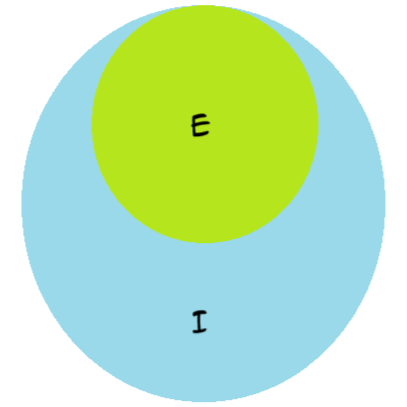
\includegraphics[scale=0.5]{phases.png}
\end{center}

When considering judgments on equality in $\top$, we need to both consider behavior and cost, which is consistent with $\top$ being dependent on judgments in $\EXT$.
In this way, we have this relationship between the phases where they are not mutually exclusive, but instead where one phase can be considered independently, while the other must be considered within the context of the first.

Similar analogies exist in other parts of language design -- for example, in a module system, we can consider solely the signature and treat the implementation as a ``black box,'' however the implementation itself is dependent on the specifications in the signature.

\subsection{Grammar}

We will formulate this system in the lax type setting, where we have terms ($\Gamma \entails \isOf{M}{A}$) and computations ($\Gamma \entails E \altDiv A$).

\[
    \begin{array}{rcl}
        \text{Computations} \quad & E ::= & \retEx*{M} \mid \bndEx*{M}{x}{E} \mid \stepEx{c}{E}\\
        \text{Terms} \quad & M ::= & \ldots \mid \compEx{E}\\
        \text{Types} \quad & A ::= & \ldots \mid \compTy{A}\\
    \end{array}
\]

There are a few things to note about the grammar:
\begin{itemize}
    \item The language now has a $\stepEx{c}{E}$ computation, which is the ``profiling'' step that records a computation of cost $c$. In the extensional phase,
    the $\kw{step}$ computation is treated as a no-op.
    \item The $c$ in the $\stepEx{c}{E}$ computation is an element of a cost monoid, $\monC$. A monoid is a set which contains an
    identity element and has an associative binary operation.
    \item You can include any other types/terms in the language as long as they are total.
\end{itemize}

\subsection{Statics}

With the new computation construct, we have a new static rule:
\begin{mathpar}
    \defrule[T-Step][sta:step]
    {c \in \monC \\ \Gamma \entails E \altDiv A}
    {\Gamma \entails \stepEx{c}{E} \altDiv A}
\end{mathpar}

The judgment $c \in \monC$ means that $c$ is an element of the cost monoid $\monC$.

\subsection{Dynamics}

For the dynamics, we have the following judgments:
\begin{enumerate}
    \item $M \evalsTo V$, to say that term $M$ evaluates to a value $V$
    \item $E \stepsToC{c} E'$, to say that a computation $E$ steps to another computation $E'$ with cost $c$ (with $c \in \monC$).
    If a step has no cost, you can simply say $E \stepsTo E'$.
\end{enumerate}

We then define the following dynamics:
\begin{mathpar}
    \defrule[D-Ret][dyn:ret]
    {M \evalsTo V}
    {\retEx*{M} \stepsTo \retEx*{V}}

    \defrule[D-Step][dyn:step]
    {\strut}
    {\stepEx{c}{E} \stepsToC{c} E}\\

    \defrule[D-Bind][dyn:bnd]
    {M \evalsTo \compEx{E_1} \\ E_1 \stepsToC{c} E_1'}
    {\bndEx*{M}{x}{E_2} \stepsToC{c} \bndEx*{\compEx{E_1'}}{x}{E_2}}

    \defrule[D-Bind-Ret][dyn:bnd-ret]
    {M \evalsTo \compEx{\retEx*{V}}}
    {\bndEx*{M}{x}{E_2} \stepsTo \Sub{V}{x}{E_2}}
\end{mathpar}

We also have the judgment $E \evalsToC{c} V$ to express that, in the complete execution of computation $E$, we reach the value $V$ (with cost $c \in \monC$).
With this judgment, we have the following dynamics:
\begin{mathpar}
    \defrule[D-Val][dyn:val]
    {M \evalsTo V}
    {\retEx*{M} \evalsToC{0} V}

    \defrule[D-Step][dyn:step2]
    {E \stepsToC{c} E' \\ E' \evalsToC{c'} V}
    {E \evalsToC{c + c'} V}
\end{mathpar}

In the second rule, $+$ is the associative binary operator that the monoid $\monC$ is equipped with.

\section{Equality and Equivalence}

When defining our equational rules for this system, we will need to now take the phase into consideration, since different phases may entail different conditions for equivalence.
We first define the judgment $\phi \entails \psi$ to mean that ``being in phase $\phi$ entails being in phase $\psi$". For example, we have that $\EXT \entails \top$. If we consider our pictorial
representation of the phases from \Cref{phases}, then this should make sense -- even though $\EXT$ can be isolated from $\top$, it is still contained
within $\top$.

For the phase entailment judgment, we have the following rules, which defines a preorder on the phases:
\begin{mathpar}
    \defrule[refl][refl]
    {\strut}
    {\phi \entails \phi}

    \defrule[Trans][trans]
    {\phi \entails \psi \\ \psi \entails \gamma}
    {\phi \entails \gamma}
\end{mathpar}

\subsection{Equality}

As one would expect, our exact equality judgments now depend on the current phase, which gives us the judgments $\exEqOfPhase{M}{M'}{A}{\phi}$ for terms and $\compEqOfPhase{E}{E'}{A}{\phi}$ for computations.

For terms, we define the judgments for $\compTy{A}$ and $\arrTy*{A_1}{A_2}$ as representative cases:
\begin{align*}
    \exEqOfPhase{M}{M'}{\compTy{A}}{\phi} &\textit{ iff } M \evalsTo \compEx*{E},\ M' \evalsTo \compEx{E'} \textit{ and } \compEqOfPhase{E}{E'}{A}{\phi}\\
    \exEqOfPhase{M}{M'}{\arrTy*{A_1}{A_2}}{\phi} &\textit{ iff }
    \begin{cases}
        M \evalsTo \lamEx*{x}{M_2},\ M' \evalsTo \lamEx*{x}{M_2'}\\
        \forall\ \psi \entails \phi, \textit{if } \exEqOfPhase{M_1}{M_1'}{A_1}{\psi}, \textit{then } \exEqOfPhase{\Sub{M_1}{x}{M_2}}{\Sub{M_1'}{x}{M_2'}}{A_2}{\psi}
    \end{cases}
\end{align*}

For computations, we define exact equality as follows:
\[\compEqOfPhase{E}{E'}{A}{\phi} \textit{ iff } \begin{cases} E \evalsToC{c} V,\ E' \evalsToC{c'} V'\\ \exEqOfPhase{V}{V'}{A}{\phi} \textit{ and either } c = c' \textit{ or } \phi \entails \EXT \end{cases}\]

More explicitly, we say that two computations are equal if they execute to the same final value with the same cost, \textit{or} we are in the extensional phase and do not need to consider cost.

\bigskip

For these judgments, we have the following anti-monotonicity lemmas:
\begin{lemma}\label{lem:anti-mono}\phantom{nextline}
    \begin{enumerate}
        \item If $\exEqOfPhase{M}{M'}{A}{\phi}$ and $\psi \entails \phi$, then $\exEqOfPhase{M}{M'}{A}{\psi}$
        \item If $\compEqOfPhase{E}{E'}{A}{\phi}$ and $\psi \entails \phi$, then $\compEqOfPhase{E}{E'}{A}{\psi}$
    \end{enumerate}
\end{lemma}

If we constrain this lemma to $\EXT \entails \top$, this would mean that any terms or computations found equal in $\top$ should also be found equal in $\EXT$,
whereas things found equal in $\EXT$ may not necessarily be equal in $\top$ (as with $\kw{msort}$ and $\kw{isort}$).

We also have head expansion for terms:
\begin{lemma}\label{lem:he}
    If $\exEqOfPhase{M}{M'}{A}{\phi}$ and $N \stepsTo M$, then $\exEqOfPhase{N}{M'}{A}{\phi}$, and if $N \stepsTo M'$, then $\exEqOfPhase{M}{N}{A}{\phi}$
\end{lemma}

Finally, we introduce new entailment judgments $\Gamma \entailsPhase{\phi} \isOf{M}{A}$ and $\Gamma \entailsPhase{\phi} E \altDiv A$ to represent entailment under a particular phase $\phi$.
We also introduce the judgment $\Gamma \gg^\phi \exEqOf{M}{M'}{A}$ (and analogously for computations), which means ``If $\exEqOfPhase{\gamma}{\gamma'}{\Gamma}{\phi}$, then $\exEqOfPhase{\gyat(M)}{\gyat'(M')}{A}{\phi}$.''
With these, we can define the reflexivity lemmas:
\begin{lemma}\label{lem:refl}\phantom{nextline}
    \begin{enumerate}
        \item If $\Gamma \entailsPhase{\phi} \isOf{M}{A}$, then $\Gamma \gg^\phi \exEqOf{M}{M}{A}$
        \item If $\Gamma \entailsPhase{\phi} E \altDiv A$, then $\Gamma \gg^\phi \compEqOf{E}{E}{A}$
    \end{enumerate}
\end{lemma}

\subsection{Equivalence}

The equivalence judgments are also dependent on the current phase, which gives us judgments of the form $\exEquivPhase{\Gamma}{\phi}{M}{M'}{A}$ for terms and
$\compEquivPhase{\Gamma}{\phi}{E}{E'}{A}$ for computations.

Since the execution steps of $\kw{ret}$ and $\kw{bind}$ do not incur cost, any equational rules not involving $\kw{step}$ will be the same as in the lax setting.
We do, however, have new equational rules for $\kw{step}$ computations:
\begin{mathpar}
    \defrule[Step-Zero][step-zero]
    {\Gamma \entailsPhase{\phi} E \altDiv A}
    {\compEquivPhase{\Gamma}{\phi}{\stepEx{0}{E}}{E}{A}}

    \defrule[Step-Step][step-step]
    {\Gamma \entailsPhase{\phi} E \altDiv A}
    {\compEquivPhase{\Gamma}{\phi}{\stepEx{c}{\stepEx{c'}{E}}}{\stepEx{c+c'}{E}}{A}}

    \defrule[Step-Ext][step-ext]
    {\Gamma \entailsPhase{\EXT} E \altDiv A}
    {\compEquivPhase{\Gamma}{\EXT}{\stepEx{c}{E}}{E}{A}}  \\

    \defrule[Step-Bind][step-bind]
    {\Gamma \entailsPhase{\phi} E_1 \altDiv A_1 \\ \Gamma, \isOf{x}{A_1} \entailsPhase{\phi} E_2 \altDiv A_2}
    {\compEquivPhase{\Gamma}{\phi}{\bndEx*{\compEx{\stepEx{c}{E_1}}}{x}{E_2}}{\stepEx{c}{\bndEx*{\compEx{E_1}}{x}{E_2}}}{A_2}}
\end{mathpar}

We might consider adding the following rule similar to the last one:

\begin{mathpar}
    \defrule[Step-Bind?][step-bind2]
    {\Gamma \entailsPhase{\phi} E_1 \altDiv A_1 \\ \Gamma, \isOf{x}{A_1} \entailsPhase{\phi} E_2 \altDiv A_2}
    {\compEquivPhase{\Gamma}{\phi}{\bndEx*{\compEx{E_1}}{x}{\stepEx{c}{E_2}}}{\stepEx{c}{\bndEx*{\compEx{E_1}}{x}{E_2}}}{A_2}}
\end{mathpar}

This rule would be permissible in the current language, however if $E_1$ diverged, then the step cost of $E_2$ would never be incurred.

\bigskip

Finally, we can state the fundamental theorems:
\begin{theorem}\label{thm:ftlr}\phantom{nextline}
    \begin{enumerate}
        \item If $\exEquivPhase{\Gamma}{\phi}{M}{M'}{A}$, then $\Gamma \gg^\phi \exEqOf{M}{M'}{A}$
        \item If $\compEquivPhase{\Gamma}{\phi}{E}{E'}{A}$, then $\Gamma \gg^\phi \compEqOf{E}{E'}{A}$
    \end{enumerate}
\end{theorem}

To prove the theorem(s), we proceed by induction on the equivalence judgment. We will prove the \textsc{Step-Bind} case of the theorem as a representative case:
\begin{proof}\phantom{nextline}\\\\
    Fix $\exEqOfPhase{\gamma}{\gamma'}{\Gamma}{\phi}$.
    We would like to show that\\ $\compEqOfPhase{\bndEx*{\compEx{\stepEx{c}{\gyat(E_1)}}}{x}{\gyat(E_2)}}{\stepEx{c}{\bndEx*{\compEx{\gyat'(E_1)}}{x}{\gyat'(E_2)}}}{A_2}{\phi}$.\\\\
    From the first premise, we have that $\Gamma \entailsPhase{\phi} E_1 \altDiv A_1$. By \Cref{lem:refl},
    we have $\compEqOfPhase{\gyat(E_1)}{\gyat'(E_1)}{A_1}{\phi}$. By definition, this means that $\gyat(E_1) \evalsToC{c_1} V_1$, $\gyat'(E_1) \evalsToC{c_1'} V_1'$ such that $\exEqOfPhase{V_1}{V_1'}{A_1}{\phi}$
    and either $c_1 = c_1'$ or $\phi \entails \EXT$.\\\\
    Consider the following stepping for both computations:
    \begin{align*}
        &\bndEx*{\compEx{\stepEx{c}{\gyat(E_1)}}}{x}{\gyat(E_2)}\\
        &\stepsToC{c} \bndEx*{\compEx{\gyat(E_1)}}{x}{\gyat(E_2)}\\
        &\evalsToC{c_1} \Sub{V_1}{x}{\gyat(E_2)}
    \end{align*}
    \begin{align*}
        &\stepEx{c}{\bndEx*{\compEx{\gyat'(E_1)}}{x}{\gyat'(E_2)}}\\
        &\stepsToC{c} \bndEx*{\compEx{\gyat'(E_1)}}{x}{\gyat'(E_2)}\\
        &\evalsToC{c_1'} \Sub{V_1'}{x}{\gyat'(E_2)}
    \end{align*}
    In other words, we have $\bndEx*{\compEx{\stepEx{c}{\gyat(E_1)}}}{x}{\gyat(E_2)} \evalsToC{c+c_1} \Sub{V_1}{x}{\gyat(E_2)}$ and $\stepEx{c}{\bndEx*{\compEx{\gyat'(E_1)}}{x}{\gyat'(E_2)}} \evalsToC{c+c_1'} \Sub{V_1'}{x}{\gyat'(E_2)}$.

    From the second premise, we have $\Gamma, \isOf{x}{A_1} \entailsPhase{\phi} E_2 \altDiv A_2$. By \Cref{lem:refl}, we would have $\compEqOfPhase{\gyat^*(E_2)}{\gyat'^*(E_2)}{A_2}{\phi}$ for $\exEqOfPhase{\gamma^*}{\gamma'^*}{\Gamma, \isOf{x}{A_1}}{\phi}$.
    Note that since $\exEqOfPhase{V_1}{V_1'}{A_1}{\phi}$ and $\exEqOfPhase{\gamma}{\gamma'}{\Gamma}{\phi}$, we have that $\compEqOfPhase{\gamma[x \mapsto V_1]}{\gamma'[x \mapsto V_1']}{\Gamma, \isOf{x}{A_1}}{\phi}$.  As such, by the result of reflexivity, we have
    $\compEqOfPhase{\widehat{\gamma[x \mapsto V_1]}(E_2)}{\widehat{\gamma'[x \mapsto V_1']}(E_2)}{A_2}{\phi}$, i.e. $\compEqOfPhase{\Sub{V_1}{x}{\gyat(E_2)}}{\Sub{V_1'}{x}{\gyat'(E_2)}}{A_2}{\phi}$ by definition of substitution.\\\\
    Since $\compEqOfPhase{\Sub{V_1}{x}{\gyat(E_2)}}{\Sub{V_1'}{x}{\gyat'(E_2)}}{A_2}{\phi}$, by definition, $\Sub{V_1}{x}{\gyat(E_2)} \evalsToC{c_2} V_2$, $\Sub{V_1'}{x}{\gyat'(E_2)} \evalsToC{c_2'} V_2'$, and either $c_2 = c_2'$ or $\phi \entails \EXT$.
    By combining these results with the previous stepping, we have $\bndEx*{\compEx{\stepEx{c}{\gyat(E_1)}}}{x}{\gyat(E_2)} \evalsToC{c + c_1 + c_2} V_2$ and $\stepEx{c}{\bndEx*{\compEx{\gyat'(E_1)}}{x}{\gyat'(E_2)}} \evalsToC{c + c_1' + c_2'} V_2'$.\\\\
    If $\phi \entails \EXT$, then we immediately have that $\compEqOfPhase{\bndEx*{\compEx{\stepEx{c}{\gyat(E_1)}}}{x}{\gyat(E_2)}}{\stepEx{c}{\bndEx*{\compEx{\gyat'(E_1)}}{x}{\gyat'(E_2)}}}{A_2}{\phi}$, since we do not need to take cost into consideration. Otherwise,
    from our previous invocations of reflexivity, we have that $c_1 = c_1'$ and $c_2 = c_2'$. Then, it follows that $c + c_1 + c_2 = c + c_1' + c_2'$.\\\\
    Thus, in either case, we have $\compEqOfPhase{\bndEx*{\compEx{\stepEx{c}{\gyat(E_1)}}}{x}{\gyat(E_2)}}{\stepEx{c}{\bndEx*{\compEx{\gyat'(E_1)}}{x}{\gyat'(E_2)}}}{A_2}{\phi}$.\\
\end{proof}

\section{Non-Interference}

In the context of extensional and intensional phases, the concept of \textit{non-interference} refers to the idea that any extensional behavior should not be affected by our intensional considerations, i.e. profiling.

The statement of the non-interference theorem is as follows:
\begin{theorem}\label{thm:non-int}
    If $\cdot \entailsPhase{\top} \isOf{F}{\normalfont\arrTy*{\compTy{\unitTy}}{\compTy{\ansTy}}}$, then $F$ is extensionally a constant function
\end{theorem}

In other words, $F$ should be extensionally equal to $\lamEx*{\_}{\compEx{\retEx*{V}}}$ for $\isOf{V}{\ansTy}$.

\begin{proof}\phantom{nextline}\\\\
To prove this, suppose we have $\cdot \entailsPhase{\top} \isOf{F}{\arrTy*{\compTy{\unitTy}}{\compTy{\ansTy}}}$. By \Cref{lem:refl}, we have that $\exEqOfPhase{F}{F}{\arrTy*{\compTy{\unitTy}}{\compTy{\ansTy}}}{\top}$.
By \Cref{lem:anti-mono}, since $\EXT \entails \top$, we have that $\exEqOfPhase{F}{F}{\arrTy*{\compTy{\unitTy}}{\compTy{\ansTy}}}{\EXT}$.\\\\
By definition of exact equality, for $\exEqOfPhase{M}{M'}{\compTy{\unitTy}}{\EXT}$, we have that $\exEqOfPhase{\appEx*{F}{M}}{\appEx*{F}{M'}}{\compTy{\ansTy}}{\phi}$.
Using that result, we have that $\appEx*{F}{M} \evalsTo \compEx{E}$, $\appEx*{F}{M'} \evalsTo \compEx{E'}$ and $\compEqOfPhase{E}{E'}{\ansTy}{\EXT}$. Additionally, since $\compEqOfPhase{E}{E'}{\ansTy}{\EXT}$, we have that
$E \evalsToC{c} V$, $E' \evalsToC{c'} V'$ such that $\exEqOfPhase{V}{V'}{\ansTy}{\EXT}$. Since $\EXT \entails \EXT$, we need not consider the cost, and we simply observe that
both functions return equal answers on equal inputs, i.e. $F$ returns either $\yesEx$ or $\noEx$. Thus, we have that $F$ is extensionally equal to $\lamEx*{\_}{\compEx{\retEx*{V}}}$ for $\isOf{V}{\ansTy}$.\\
\end{proof}

\end{document}
